%%%%%%%%%%%%%%%%%%%%%%%%%%%%%%%%%%%%%%%%%
% a0poster Landscape Poster
% LaTeX Template
% Version 1.0 (22/06/13)
%
% The a0poster class was created by:
% Gerlinde Kettl and Matthias Weiser (tex@kettl.de)
% 
% This template has been downloaded from:
% http://www.LaTeXTemplates.com
%
% License:
% CC BY-NC-SA 3.0 (http://creativecommons.org/licenses/by-nc-sa/3.0/)
%
%%%%%%%%%%%%%%%%%%%%%%%%%%%%%%%%%%%%%%%%%

%----------------------------------------------------------------------------------------
%	PACKAGES AND OTHER DOCUMENT CONFIGURATIONS
%----------------------------------------------------------------------------------------

\documentclass[a0,landscape]{a0poster}

\usepackage{multicol} % This is so we can have multiple columns of text side-by-side
\columnsep=100pt % This is the amount of white space between the columns in the poster
\columnseprule=3pt % This is the thickness of the black line between the columns in the poster

\usepackage[svgnames]{xcolor} % Specify colors by their 'svgnames', for a full list of all colors available see here: http://www.latextemplates.com/svgnames-colors

\usepackage{times} % Use the times font
%\usepackage{palatino} % Uncomment to use the Palatino font

\usepackage{graphicx} % Required for including images
\graphicspath{{figures/}} % Location of the graphics files
\usepackage{booktabs} % Top and bottom rules for table
\usepackage[font=small,labelfont=bf]{caption} % Required for specifying captions to tables and figures
\usepackage{amsfonts, amsmath, amsthm, amssymb} % For math fonts, symbols and environments
\usepackage{wrapfig} % Allows wrapping text around tables and figures

% For more fonts: see http://www.tug.dk/FontCatalogue/allfonts.html
%\input ArtNouvc.fd
%\newcommand*\initfamily{\usefont{U}{ArtNouvc}{xl}{n}}
%\input Acorn.fd
%\newcommand*\initfamily{\usefont{U}{Acorn}{xl}{n}}
\input Kinigcap.fd
\newcommand*\initfamily{\usefont{U}{Kinigcap}{xl}{n}}
%\input Sanremo.fd
%\newcommand*\initfamily{\usefont{U}{Sanremo}{xl}{n}}
%\input Starburst.fd
%\newcommand*\initfamily{\usefont{U}{Starburst}{xl}{n}}
\definecolor{supercolor}{rgb}{0.1, 0.188, 1}



\begin{document}

%----------------------------------------------------------------------------------------
%	POSTER HEADER 
%----------------------------------------------------------------------------------------

% The header is divided into three boxes:
% The first is 55% wide and houses the title, subtitle, names and university/organization
% The second is 25% wide and houses contact information
% The third is 19% wide and houses a logo for your university/organization or a photo of you
% The widths of these boxes can be easily edited to accommodate your content as you see fit

\begin{minipage}[b]{0.48\linewidth}
\veryHuge \color{NavyBlue} \textbf{PlayCDC - Playing Card Detection} \color{Black}\\ % Title
\Huge\textit{Learning to detect suits and ranks of playing cards}\\[1cm] % Subtitle
\huge \textbf{Daniel Gonzalez \& Frank Gabel}\\ % Author(s)
\huge Ruprecht-Karls-Universit\"at Heidelberg
\\ % University/organization
\end{minipage}
%
\begin{minipage}[b]{0.17\linewidth}
\color{DarkSlateGray}\Large \textbf{Contact Information:}\\
Daniel Gonzalez\\ % Name
Email: \texttt{d.gonzalez@stud.uni-heidelberg.de}\
\\\\
Frank Gabel \\
%Phone: +1 (000) 111 1111\\ % Phone number
Email: \texttt{ey143@uni-heidelberg.de}\\ % Email address
\end{minipage}
%
\begin{minipage}[b]{0.49\linewidth}
\quad \center \textcolor{supercolor} {\fontsize{140}{50} \initfamily PLAYCDC} \vspace{4cm}
%
\includegraphics[width=30cm]{playcdc.png} % Logo or a photo of you, adjust its dimensions here
\end{minipage}

\vspace{1cm} % A bit of extra whitespace between the header and poster content

%----------------------------------------------------------------------------------------

\begin{multicols}{3} % This is how many columns your poster will be broken into, a poster with many figures may benefit from less columns whereas a text-heavy poster benefits from more

%----------------------------------------------------------------------------------------
%	ABSTRACT
%----------------------------------------------------------------------------------------

\color{Navy} % Navy color for the abstract

\begin{abstract}

With the capabilities of upcoming small video capturing devices in, for example, smart contact lenses with built-in camerass, whole new ways of cheating in certain cardgames emerge. In order to help facilitate these cheating endeavours, we implement an algorithm that detects the suits and ranks of playing cards in the field of view of a camera using the latest iteration of the YOLO object recognition algorithm.


\end{abstract}

%----------------------------------------------------------------------------------------
%	INTRODUCTION
%----------------------------------------------------------------------------------------

\color{SaddleBrown} % SaddleBrown color for the introduction

\section*{Introduction}
Object detection deals with detecting instances of semantic objects of a certain class (such as humans, buildings, or cars) in digital images and videos. 


%----------------------------------------------------------------------------------------
%	OBJECTIVES
%----------------------------------------------------------------------------------------

\color{DarkSlateGray} % DarkSlateGray color for the rest of the content

\section*{Main Objectives}
The objectives of this project are summarized as follows:

\begin{description}

\item[Create a general dataset] of a standard, 52-card deck of playing cards  in different poses, brightness situations and blurring levels annotated with bounding boxes around the ranks and suits and corresponding class information.
\item[Train an object detection algorithm] on these synthesized data that performs bounding box localization and regression for classification. In particular, we train  the latest iteration of the YOLO object detection algorithm \cite{DBLP:journals/corr/abs-1804-02767} end-to-end.
\item[Evaluate the algorithm on a hold-out validation dataset] covering all classes. As a performance metric, mean Average Precision (mAP) is used.
\item[Deploy the model on a smartphone camera] as a proof of concept.

\end{description}


%----------------------------------------------------------------------------------------
%	MATERIALS AND METHODS
%----------------------------------------------------------------------------------------

\section*{Methods}
\subsection*{The dataset creation pipeline}
The dataset was created in manly 2 big steps. \\
First, we took two photos for each card in a deck of 52 cards, crop the cards to a selection and rescale the result by 600x900 pixels.
This was done manually using  the selection/rotation/cropping/re-scale -tools provided by GIMP.  Concluding this, we manage to detect the convex hulls of the
cards suits and  ranks using the SciPy library.  \\
The next step was to generate a big amount of data for each card applying linear transfomations, as well as blurring and sharping on the image.
First we paste the images in canvances using the Describable Textures Dataset [cite], in order to have different textures arround the image.
For the next, we use the imgaug library in order to perform the mentioned transformations, keeping track of the convex hulls. \\
For each of the 52 cards of the deck, we generate in total 450 images for trainig. 




% IMAGES
% \centering\vspace{1cm}
 %	\begin{minipage}[b]{0.16\textwidth}
  % 		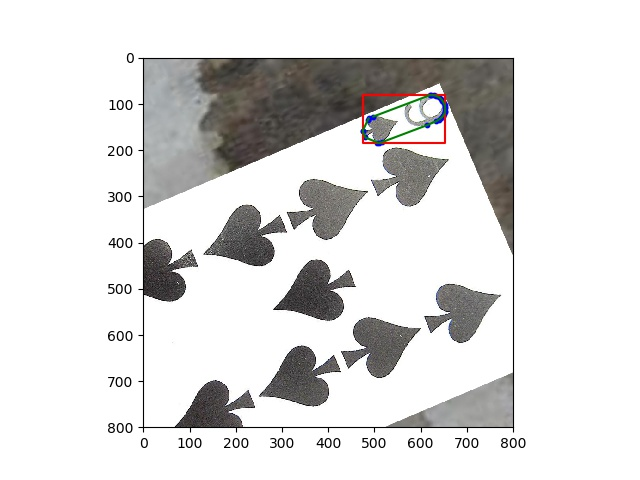
\includegraphics[width=\textwidth]{7-full}
%		\captionof{figure}{\color{Green} Figure caption}
% 	 \end{minipage}
% \hspace{2cm}
% 	\begin{minipage}[b]{0.12\textwidth}
 %  		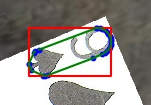
\includegraphics[width=\textwidth]{7}
%		\captionof{figure}{\color{Green} Figure caption}
% 	\end{minipage}\vspace{1cm}

\centering\vspace{1cm}
\begin{minipage}[b]{0.25\textwidth}
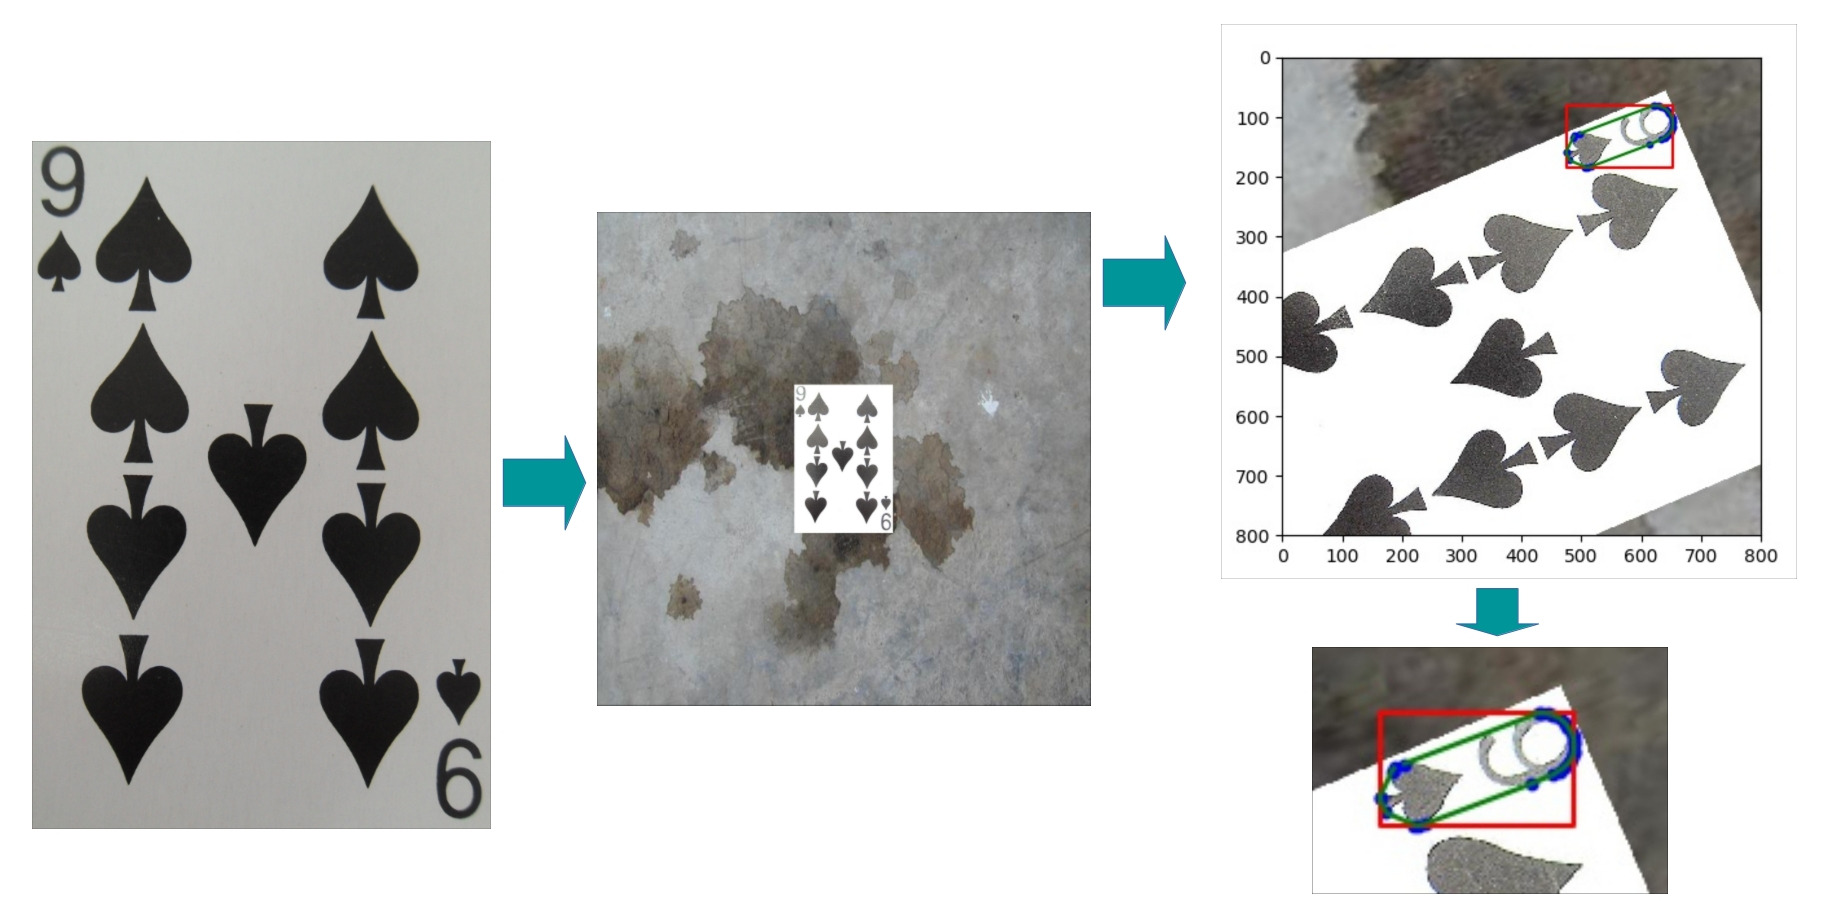
\includegraphics[width=\textwidth]{7-p}
\captionof{figure}{\color{Green} Figure caption}
\end{minipage}
%\begin{center}\vspace{1cm}
%
\includegraphics[width=0.5\linewidth]{placeholder}
%\captionof{figure}{\color{Green} Figure caption}
%\end{center}\vspace{1cm}
%------------------------------------------------

\subsection*{The tiny-YOLO-v3 object detection algorithm}

Nulla vel nisl sed mauris auctor mollis non sed. 
\subsection*{Evaluation strategy}
\begin{equation}
E = mc^{2}
\label{eqn:Einstein}
\end{equation}

Curabitur mi sem, pulvinar quis aliquam rutrum. (1) edf (2)
, $\Omega=[-1,1]^3$, maecenas leo est, ornare at. $z=-1$ edf $z=1$ sed interdum felis dapibus sem. $x$ set $y$ ytruem. 
Turpis $j$ amet accumsan enim $y$-lacina; 
ref $k$-viverra nec porttitor $x$-lacina. 

Vestibulum ac diam a odio tempus congue. Vivamus id enim nisi:

\begin{eqnarray}
\cos\bar{\phi}_k Q_{j,k+1,t} + Q_{j,k+1,x}+\frac{\sin^2\bar{\phi}_k}{T\cos\bar{\phi}_k} Q_{j,k+1} &=&\nonumber\\ 
-\cos\phi_k Q_{j,k,t} + Q_{j,k,x}-\frac{\sin^2\phi_k}{T\cos\phi_k} Q_{j,k}\label{edgek}
\end{eqnarray}
and
\begin{eqnarray}
\cos\bar{\phi}_j Q_{j+1,k,t} + Q_{j+1,k,y}+\frac{\sin^2\bar{\phi}_j}{T\cos\bar{\phi}_j} Q_{j+1,k}&=&\nonumber \\
-\cos\phi_j Q_{j,k,t} + Q_{j,k,y}-\frac{\sin^2\phi_j}{T\cos\phi_j} Q_{j,k}.\label{edgej}
\end{eqnarray} 


%----------------------------------------------------------------------------------------
%	RESULTS 
%----------------------------------------------------------------------------------------

\section*{Results}

Donec faucibus purus at tortor egestas eu fermentum dolor facilisis. Maecenas tempor dui eu neque fringilla rutrum. Mauris \emph{lobortis} nisl accumsan. Aenean vitae risus ante. Pellentesque condimentum dui. Etiam sagittis purus non tellus tempor volutpat. Donec et dui non massa tristique adipiscing.
%
\begin{wraptable}{l}{12cm} % Left or right alignment is specified in the first bracket, the width of the table is in the second
\begin{tabular}{l l l}
\toprule
\textbf{Treatments} & \textbf{Response 1} & \textbf{Response 2}\\
\midrule
Treatment 1 & 0.0003262 & 0.562 \\
Treatment 2 & 0.0015681 & 0.910 \\
Treatment 3 & 0.0009271 & 0.296 \\
\bottomrule
\end{tabular}
\captionof{table}{\color{Green} Table caption}
\end{wraptable}
%
Phasellus imperdiet, tortor vitae congue bibendum, felis enim sagittis lorem, et volutpat ante orci sagittis mi. Morbi rutrum laoreet semper. Morbi accumsan enim nec tortor consectetur non commodo nisi sollicitudin. Proin sollicitudin. Pellentesque eget orci eros. Fusce ultricies, tellus et pellentesque fringilla, ante massa luctus libero, quis tristique purus urna nec nibh.

Nulla ut porttitor enim. Suspendisse venenatis dui eget eros gravida tempor. Mauris feugiat elit et augue placerat ultrices. Morbi accumsan enim nec tortor consectetur non commodo. Pellentesque condimentum dui. Etiam sagittis purus non tellus tempor volutpat. Donec et dui non massa tristique adipiscing. Quisque vestibulum eros eu. Phasellus imperdiet, tortor vitae congue bibendum, felis enim sagittis lorem, et volutpat ante orci sagittis mi. Morbi rutrum laoreet semper. Morbi accumsan enim nec tortor consectetur non commodo nisi sollicitudin.

\begin{center}\vspace{1cm}

\includegraphics[width=0.8\linewidth]{placeholder}
\captionof{figure}{\color{Green} Figure caption}
\end{center}\vspace{1cm}

In hac habitasse platea dictumst. Etiam placerat, risus ac.

Adipiscing lectus in magna blandit:

\begin{center}\vspace{1cm}
\begin{tabular}{l l l l}
\toprule
\textbf{Treatments} & \textbf{Response 1} & \textbf{Response 2} \\
\midrule
Treatment 1 & 0.0003262 & 0.562 \\
Treatment 2 & 0.0015681 & 0.910 \\
Treatment 3 & 0.0009271 & 0.296 \\
\bottomrule
\end{tabular}
\captionof{table}{\color{Green} Table caption}
\end{center}\vspace{1cm}

Vivamus sed nibh ac metus tristique tristique a vitae ante. Sed lobortis mi ut arcu fringilla et adipiscing ligula rutrum. Aenean turpis velit, placerat eget tincidunt nec, ornare in nisl. In placerat.

\begin{center}\vspace{1cm}

\includegraphics[width=0.8\linewidth]{placeholder}
\captionof{figure}{\color{Green} Figure caption}
\end{center}\vspace{1cm}

%----------------------------------------------------------------------------------------
%	CONCLUSIONS
%----------------------------------------------------------------------------------------

\color{SaddleBrown} % SaddleBrown color for the conclusions to make them stand out

\section*{Conclusions}

\begin{itemize}
\item Using an artificially created dataset, we achieve a mAP score of 95.10\% on a holdout dataset.
\item The task of object detection on ranks/suits of playing cards appears to be rather easy - it can be thought of being 2D rather than 3D.
\item Deploying the model on a webcam results in 180 FPS on a 480x480 resolution, which is state-of-the-art fast.

\end{itemize}

\color{DarkSlateGray} % Set the color back to DarkSlateGray for the rest of the content

%----------------------------------------------------------------------------------------
%	FORTHCOMING RESEARCH
%----------------------------------------------------------------------------------------

\section*{Forthcoming Research}

Vivamus molestie, risus tempor vehicula mattis, libero arcu volutpat purus, sed blandit sem nibh eget turpis. Maecenas rutrum dui blandit lorem vulputate gravida. Praesent venenatis mi vel lorem tempor at varius diam sagittis. Nam eu leo id turpis interdum luctus a sed augue. Nam tellus.

 %----------------------------------------------------------------------------------------
%	REFERENCES
%----------------------------------------------------------------------------------------

\nocite{*} % Print all references regardless of whether they were cited in the poster or not
\bibliographystyle{alpha} % Plain referencing style
\bibliography{sample} % Use the example bibliography file sample.bib

%----------------------------------------------------------------------------------------
%	ACKNOWLEDGEMENTS
%----------------------------------------------------------------------------------------

\section*{Acknowledgements}

Etiam fermentum, arcu ut gravida fringilla, dolor arcu laoreet justo, ut imperdiet urna arcu a arcu. Donec nec ante a dui tempus consectetur. Cras nisi turpis, dapibus sit amet mattis sed, laoreet.

%----------------------------------------------------------------------------------------

\end{multicols}
\end{document}